\documentclass[twoside]{book}

% Packages required by doxygen
\usepackage{fixltx2e}
\usepackage{calc}
\usepackage{doxygen}
\usepackage[export]{adjustbox} % also loads graphicx
\usepackage{graphicx}
\usepackage[utf8]{inputenc}
\usepackage{makeidx}
\usepackage{multicol}
\usepackage{multirow}
\PassOptionsToPackage{warn}{textcomp}
\usepackage{textcomp}
\usepackage[nointegrals]{wasysym}
\usepackage[table]{xcolor}

% NLS support packages
\usepackage[T2A]{fontenc}
\usepackage[russian]{babel}

% Font selection
\usepackage[T1]{fontenc}
\usepackage[scaled=.90]{helvet}
\usepackage{courier}
\usepackage{amssymb}
\usepackage{sectsty}
\renewcommand{\familydefault}{\sfdefault}
\allsectionsfont{%
  \fontseries{bc}\selectfont%
  \color{darkgray}%
}
\renewcommand{\DoxyLabelFont}{%
  \fontseries{bc}\selectfont%
  \color{darkgray}%
}
\newcommand{\+}{\discretionary{\mbox{\scriptsize$\hookleftarrow$}}{}{}}

% Page & text layout
\usepackage{geometry}
\geometry{%
  a4paper,%
  top=2.5cm,%
  bottom=2.5cm,%
  left=2.5cm,%
  right=2.5cm%
}
\tolerance=750
\hfuzz=15pt
\hbadness=750
\setlength{\emergencystretch}{15pt}
\setlength{\parindent}{0cm}
\setlength{\parskip}{3ex plus 2ex minus 2ex}
\makeatletter
\renewcommand{\paragraph}{%
  \@startsection{paragraph}{4}{0ex}{-1.0ex}{1.0ex}{%
    \normalfont\normalsize\bfseries\SS@parafont%
  }%
}
\renewcommand{\subparagraph}{%
  \@startsection{subparagraph}{5}{0ex}{-1.0ex}{1.0ex}{%
    \normalfont\normalsize\bfseries\SS@subparafont%
  }%
}
\makeatother

% Headers & footers
\usepackage{fancyhdr}
\pagestyle{fancyplain}
\fancyhead[LE]{\fancyplain{}{\bfseries\thepage}}
\fancyhead[CE]{\fancyplain{}{}}
\fancyhead[RE]{\fancyplain{}{\bfseries\leftmark}}
\fancyhead[LO]{\fancyplain{}{\bfseries\rightmark}}
\fancyhead[CO]{\fancyplain{}{}}
\fancyhead[RO]{\fancyplain{}{\bfseries\thepage}}
\fancyfoot[LE]{\fancyplain{}{}}
\fancyfoot[CE]{\fancyplain{}{}}
\fancyfoot[RE]{\fancyplain{}{\bfseries\scriptsize Создано системой Doxygen }}
\fancyfoot[LO]{\fancyplain{}{\bfseries\scriptsize Создано системой Doxygen }}
\fancyfoot[CO]{\fancyplain{}{}}
\fancyfoot[RO]{\fancyplain{}{}}
\renewcommand{\footrulewidth}{0.4pt}
\renewcommand{\chaptermark}[1]{%
  \markboth{#1}{}%
}
\renewcommand{\sectionmark}[1]{%
  \markright{\thesection\ #1}%
}

% Indices & bibliography
\usepackage{natbib}
\usepackage[titles]{tocloft}
\setcounter{tocdepth}{3}
\setcounter{secnumdepth}{5}
\makeindex

% Hyperlinks (required, but should be loaded last)
\usepackage{ifpdf}
\ifpdf
  \usepackage[pdftex,pagebackref=true]{hyperref}
\else
  \usepackage[ps2pdf,pagebackref=true]{hyperref}
\fi
\hypersetup{%
  colorlinks=true,%
  linkcolor=blue,%
  citecolor=blue,%
  unicode%
}

% Custom commands
\newcommand{\clearemptydoublepage}{%
  \newpage{\pagestyle{empty}\cleardoublepage}%
}

\usepackage{caption}
\captionsetup{labelsep=space,justification=centering,font={bf},singlelinecheck=off,skip=4pt,position=top}

%===== C O N T E N T S =====

\begin{document}

% Titlepage & ToC
\hypersetup{pageanchor=false,
             bookmarksnumbered=true,
             pdfencoding=unicode
            }
\pagenumbering{alph}
\begin{titlepage}
\vspace*{7cm}
\begin{center}%
{\Large Radix }\\
\vspace*{1cm}
{\large Создано системой Doxygen 1.8.13}\\
\end{center}
\end{titlepage}
\clearemptydoublepage
\pagenumbering{roman}
\tableofcontents
\clearemptydoublepage
\pagenumbering{arabic}
\hypersetup{pageanchor=true}

%--- Begin generated contents ---
\chapter{Список файлов}
\section{Файлы}
Полный список документированных файлов.\begin{DoxyCompactList}
\item\contentsline{section}{{\bfseries Checking\+Connections.\+h} }{\pageref{_checking_connections_8h}}{}
\item\contentsline{section}{{\bfseries Checking\+Menu.\+h} }{\pageref{_checking_menu_8h}}{}
\item\contentsline{section}{\hyperlink{_initialization_8cpp}{Initialization.\+cpp} \\*Модуль проверки стандартных файлов программы }{\pageref{_initialization_8cpp}}{}
\item\contentsline{section}{\hyperlink{_initialization_8h}{Initialization.\+h} \\*Заголовочный файл с вызовом модуля инициализации }{\pageref{_initialization_8h}}{}
\item\contentsline{section}{\hyperlink{_logger_8cpp}{Logger.\+cpp} \\*Модуль логирования }{\pageref{_logger_8cpp}}{}
\item\contentsline{section}{\hyperlink{_logger_8h}{Logger.\+h} \\*Заголовочный файл с подключением модуля логирования }{\pageref{_logger_8h}}{}
\item\contentsline{section}{\hyperlink{_main_8cpp}{Main.\+cpp} \\*Главный файл программы }{\pageref{_main_8cpp}}{}
\item\contentsline{section}{{\bfseries Main\+Menu.\+h} }{\pageref{_main_menu_8h}}{}
\item\contentsline{section}{{\bfseries Net.\+h} }{\pageref{_net_8h}}{}
\item\contentsline{section}{\hyperlink{_radix_8cpp}{Radix.\+cpp} \\*Главный файл программы }{\pageref{_radix_8cpp}}{}
\item\contentsline{section}{\hyperlink{_radix_8h}{Radix.\+h} \\*Заголовочный файл с вызовом главной функции программы }{\pageref{_radix_8h}}{}
\item\contentsline{section}{\hyperlink{_settings_8cpp}{Settings.\+cpp} \\*Модуль настроек. Парсит переменные в файлах }{\pageref{_settings_8cpp}}{}
\item\contentsline{section}{\hyperlink{_settings_8h}{Settings.\+h} \\*Заголовочный файл с подключением модуля настроек }{\pageref{_settings_8h}}{}
\item\contentsline{section}{\hyperlink{_templates_8cpp}{Templates.\+cpp} \\*Функции для создания стандартных файлов программы }{\pageref{_templates_8cpp}}{}
\item\contentsline{section}{\hyperlink{_templates_8h}{Templates.\+h} \\*Заголовочный файл с подключением модуля создания стандартных файлов программы }{\pageref{_templates_8h}}{}
\end{DoxyCompactList}

\chapter{Файлы}
\hypertarget{_checking_connections_8cpp}{}\section{Файл Checking\+Connections.\+cpp}
\label{_checking_connections_8cpp}\index{Checking\+Connections.\+cpp@{Checking\+Connections.\+cpp}}


Модуль проверки соединения.  


\subsection*{Функции}
\begin{DoxyCompactItemize}
\item 
bool \hyperlink{_checking_connections_8cpp_aa1e4924f4faf010e0b60e880f1bfd7dc}{b\+\_\+checkingconnections\+\_\+phone} ()
\item 
bool \hyperlink{_checking_connections_8cpp_a5db9a9ba779bd41fe05c5b402e770732}{b\+\_\+checkingconnections\+\_\+internet} ()
\end{DoxyCompactItemize}


\subsection{Подробное описание}
Модуль проверки соединения. 

\begin{DoxyAuthor}{Автор}
Sava\+Lione 
\end{DoxyAuthor}


\subsection{Функции}
\mbox{\Hypertarget{_checking_connections_8cpp_a5db9a9ba779bd41fe05c5b402e770732}\label{_checking_connections_8cpp_a5db9a9ba779bd41fe05c5b402e770732}} 
\index{Checking\+Connections.\+cpp@{Checking\+Connections.\+cpp}!b\+\_\+checkingconnections\+\_\+internet@{b\+\_\+checkingconnections\+\_\+internet}}
\index{b\+\_\+checkingconnections\+\_\+internet@{b\+\_\+checkingconnections\+\_\+internet}!Checking\+Connections.\+cpp@{Checking\+Connections.\+cpp}}
\subsubsection{\texorpdfstring{b\+\_\+checkingconnections\+\_\+internet()}{b\_checkingconnections\_internet()}}
{\footnotesize\ttfamily bool b\+\_\+checkingconnections\+\_\+internet (\begin{DoxyParamCaption}{ }\end{DoxyParamCaption})}

Проверка соединения с интернетом. \begin{DoxyReturn}{Возвращает}
true, если соединение есть. false, если соединения нет. 
\end{DoxyReturn}
\mbox{\Hypertarget{_checking_connections_8cpp_aa1e4924f4faf010e0b60e880f1bfd7dc}\label{_checking_connections_8cpp_aa1e4924f4faf010e0b60e880f1bfd7dc}} 
\index{Checking\+Connections.\+cpp@{Checking\+Connections.\+cpp}!b\+\_\+checkingconnections\+\_\+phone@{b\+\_\+checkingconnections\+\_\+phone}}
\index{b\+\_\+checkingconnections\+\_\+phone@{b\+\_\+checkingconnections\+\_\+phone}!Checking\+Connections.\+cpp@{Checking\+Connections.\+cpp}}
\subsubsection{\texorpdfstring{b\+\_\+checkingconnections\+\_\+phone()}{b\_checkingconnections\_phone()}}
{\footnotesize\ttfamily bool b\+\_\+checkingconnections\+\_\+phone (\begin{DoxyParamCaption}{ }\end{DoxyParamCaption})}

Проверка телефона через adb. \begin{DoxyReturn}{Возвращает}
true, если телефон подключен. false, если телефон не подключен. 
\end{DoxyReturn}

\hypertarget{_checking_connections_8h}{}\section{Файл Checking\+Connections.\+h}
\label{_checking_connections_8h}\index{Checking\+Connections.\+h@{Checking\+Connections.\+h}}


Заголовочный файл с подключением модуля проверки соединения.  


\subsection*{Функции}
\begin{DoxyCompactItemize}
\item 
bool \hyperlink{_checking_connections_8h_aa1e4924f4faf010e0b60e880f1bfd7dc}{b\+\_\+checkingconnections\+\_\+phone} ()
\item 
bool \hyperlink{_checking_connections_8h_a5db9a9ba779bd41fe05c5b402e770732}{b\+\_\+checkingconnections\+\_\+internet} ()
\end{DoxyCompactItemize}


\subsection{Подробное описание}
Заголовочный файл с подключением модуля проверки соединения. 

\begin{DoxyAuthor}{Автор}
Sava\+Lione 
\end{DoxyAuthor}


\subsection{Функции}
\mbox{\Hypertarget{_checking_connections_8h_a5db9a9ba779bd41fe05c5b402e770732}\label{_checking_connections_8h_a5db9a9ba779bd41fe05c5b402e770732}} 
\index{Checking\+Connections.\+h@{Checking\+Connections.\+h}!b\+\_\+checkingconnections\+\_\+internet@{b\+\_\+checkingconnections\+\_\+internet}}
\index{b\+\_\+checkingconnections\+\_\+internet@{b\+\_\+checkingconnections\+\_\+internet}!Checking\+Connections.\+h@{Checking\+Connections.\+h}}
\subsubsection{\texorpdfstring{b\+\_\+checkingconnections\+\_\+internet()}{b\_checkingconnections\_internet()}}
{\footnotesize\ttfamily bool b\+\_\+checkingconnections\+\_\+internet (\begin{DoxyParamCaption}{ }\end{DoxyParamCaption})}

Проверка соединения с интернетом. \begin{DoxyReturn}{Возвращает}
true, если соединение есть. false, если соединения нет. 
\end{DoxyReturn}
\mbox{\Hypertarget{_checking_connections_8h_aa1e4924f4faf010e0b60e880f1bfd7dc}\label{_checking_connections_8h_aa1e4924f4faf010e0b60e880f1bfd7dc}} 
\index{Checking\+Connections.\+h@{Checking\+Connections.\+h}!b\+\_\+checkingconnections\+\_\+phone@{b\+\_\+checkingconnections\+\_\+phone}}
\index{b\+\_\+checkingconnections\+\_\+phone@{b\+\_\+checkingconnections\+\_\+phone}!Checking\+Connections.\+h@{Checking\+Connections.\+h}}
\subsubsection{\texorpdfstring{b\+\_\+checkingconnections\+\_\+phone()}{b\_checkingconnections\_phone()}}
{\footnotesize\ttfamily bool b\+\_\+checkingconnections\+\_\+phone (\begin{DoxyParamCaption}{ }\end{DoxyParamCaption})}

Проверка телефона через adb. \begin{DoxyReturn}{Возвращает}
true, если телефон подключен. false, если телефон не подключен. 
\end{DoxyReturn}

\hypertarget{_download_8cpp}{}\section{Файл Download.\+cpp}
\label{_download_8cpp}\index{Download.\+cpp@{Download.\+cpp}}


Модуль загрузки. Загружает файл  


{\ttfamily \#include $<$urlmon.\+h$>$}\newline
{\ttfamily \#include $<$Windows.\+h$>$}\newline
{\ttfamily \#include $<$string$>$}\newline
{\ttfamily \#include $<$iostream$>$}\newline
{\ttfamily \#include \char`\"{}Ip.\+h\char`\"{}}\newline
{\ttfamily \#include \char`\"{}Logger.\+h\char`\"{}}\newline
{\ttfamily \#include \char`\"{}..\textbackslash{}core\textbackslash{}\+Constants.\+h\char`\"{}}\newline
Граф включаемых заголовочных файлов для Download.\+cpp\+:\nopagebreak
\begin{figure}[H]
\begin{center}
\leavevmode
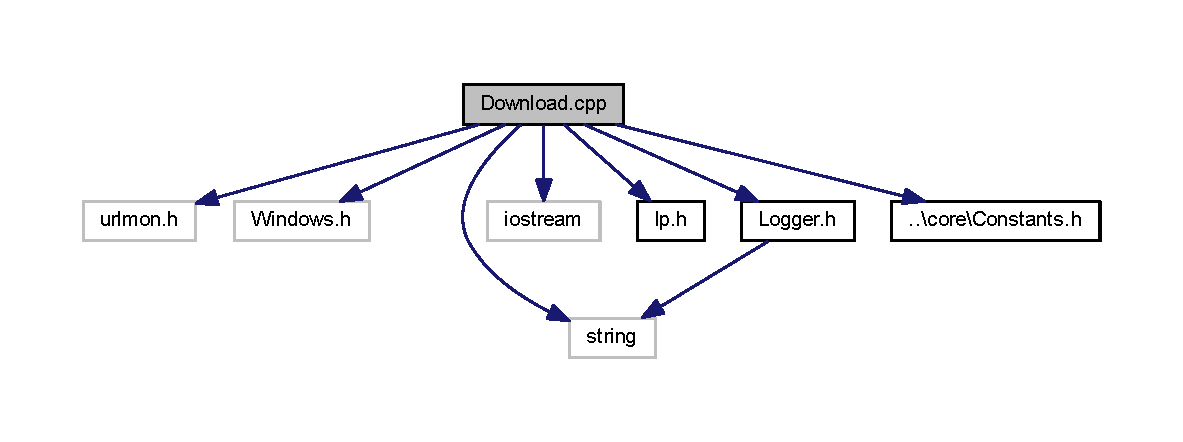
\includegraphics[width=350pt]{_download_8cpp__incl}
\end{center}
\end{figure}
\subsection*{Функции}
\begin{DoxyCompactItemize}
\item 
std\+::wstring \hyperlink{_download_8cpp_ae9cab0756619dfee595d5b254cfc4859}{s2ws} (const std\+::string \&s)
\item 
void \hyperlink{_download_8cpp_ab3291bd9df2e78c286f024fb1df3a683}{v\+\_\+download\+\_\+file} (char $\ast$ch\+\_\+file)
\end{DoxyCompactItemize}


\subsection{Подробное описание}
Модуль загрузки. Загружает файл 

\begin{DoxyAuthor}{Автор}
Sava\+Lione 
\end{DoxyAuthor}


\subsection{Функции}
\mbox{\Hypertarget{_download_8cpp_ae9cab0756619dfee595d5b254cfc4859}\label{_download_8cpp_ae9cab0756619dfee595d5b254cfc4859}} 
\index{Download.\+cpp@{Download.\+cpp}!s2ws@{s2ws}}
\index{s2ws@{s2ws}!Download.\+cpp@{Download.\+cpp}}
\subsubsection{\texorpdfstring{s2ws()}{s2ws()}}
{\footnotesize\ttfamily std\+::wstring s2ws (\begin{DoxyParamCaption}\item[{const std\+::string \&}]{s }\end{DoxyParamCaption})}

Преобразование типа string к типу wstring 
\begin{DoxyParams}[1]{Аргументы}
\mbox{\tt in}  & {\em s} & ссылка на строку string \\
\hline
\end{DoxyParams}
\begin{DoxyReturn}{Возвращает}
wstring 
\end{DoxyReturn}
\mbox{\Hypertarget{_download_8cpp_ab3291bd9df2e78c286f024fb1df3a683}\label{_download_8cpp_ab3291bd9df2e78c286f024fb1df3a683}} 
\index{Download.\+cpp@{Download.\+cpp}!v\+\_\+download\+\_\+file@{v\+\_\+download\+\_\+file}}
\index{v\+\_\+download\+\_\+file@{v\+\_\+download\+\_\+file}!Download.\+cpp@{Download.\+cpp}}
\subsubsection{\texorpdfstring{v\+\_\+download\+\_\+file()}{v\_download\_file()}}
{\footnotesize\ttfamily void v\+\_\+download\+\_\+file (\begin{DoxyParamCaption}\item[{char $\ast$}]{ch\+\_\+file }\end{DoxyParamCaption})}

Загрузка файла по уникальному номеру 
\begin{DoxyParams}[1]{Аргументы}
\mbox{\tt in}  & {\em ch\+\_\+file} & Номер файла для загрузки \\
\hline
\end{DoxyParams}
\begin{Desc}
\item[Примеры\+: ]\par
\hyperlink{v_download_file_8cpp-example}{v\+\_\+download\+\_\+file.\+cpp}.\end{Desc}

\hypertarget{_download_8h}{}\section{Файл Download.\+h}
\label{_download_8h}\index{Download.\+h@{Download.\+h}}


Заголовочный файл с подключением модуля загрузки файла.  


\subsection*{Функции}
\begin{DoxyCompactItemize}
\item 
void \hyperlink{_download_8h_a650610c34115bb7f006e260d3d492382}{v\+\_\+download\+\_\+file} (size\+\_\+t sz\+\_\+file)
\end{DoxyCompactItemize}


\subsection{Подробное описание}
Заголовочный файл с подключением модуля загрузки файла. 

\begin{DoxyAuthor}{Автор}
Sava\+Lione 
\end{DoxyAuthor}


\subsection{Функции}
\mbox{\Hypertarget{_download_8h_a650610c34115bb7f006e260d3d492382}\label{_download_8h_a650610c34115bb7f006e260d3d492382}} 
\index{Download.\+h@{Download.\+h}!v\+\_\+download\+\_\+file@{v\+\_\+download\+\_\+file}}
\index{v\+\_\+download\+\_\+file@{v\+\_\+download\+\_\+file}!Download.\+h@{Download.\+h}}
\subsubsection{\texorpdfstring{v\+\_\+download\+\_\+file()}{v\_download\_file()}}
{\footnotesize\ttfamily void v\+\_\+download\+\_\+file (\begin{DoxyParamCaption}\item[{size\+\_\+t}]{sz\+\_\+file }\end{DoxyParamCaption})}

Загрузка файла по уникальному номеру 
\begin{DoxyParams}[1]{Аргументы}
\mbox{\tt in}  & {\em sz\+\_\+file} & Номер файла для загрузки \\
\hline
\end{DoxyParams}

\hypertarget{_initialization_8cpp}{}\section{Файл Initialization.\+cpp}
\label{_initialization_8cpp}\index{Initialization.\+cpp@{Initialization.\+cpp}}


Модуль проверки стандартных файлов программы.  


{\ttfamily \#include $<$fstream$>$}\newline
{\ttfamily \#include \char`\"{}..\textbackslash{}io\textbackslash{}\+Templates.\+h\char`\"{}}\newline
{\ttfamily \#include \char`\"{}..\textbackslash{}io\textbackslash{}\+Logger.\+h\char`\"{}}\newline
{\ttfamily \#include \char`\"{}Constants.\+h\char`\"{}}\newline
{\ttfamily \#include \char`\"{}..\textbackslash{}ui\textbackslash{}\+Load\+Scale.\+h\char`\"{}}\newline
Граф включаемых заголовочных файлов для Initialization.\+cpp\+:
\nopagebreak
\begin{figure}[H]
\begin{center}
\leavevmode
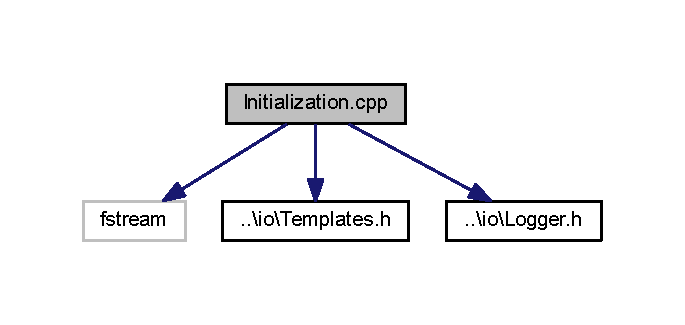
\includegraphics[width=350pt]{_initialization_8cpp__incl}
\end{center}
\end{figure}
\subsection*{Функции}
\begin{DoxyCompactItemize}
\item 
void \hyperlink{_initialization_8cpp_a61271965777637ec3d70f6d7ab0a466a}{v\+\_\+initialization\+\_\+logger\+\_\+log} ()
\begin{DoxyCompactList}\small\item\em Проверка файла logger.\+log. \end{DoxyCompactList}\item 
void \hyperlink{_initialization_8cpp_a86860ef24d9abdaddea8e817e84528a7}{v\+\_\+initialization\+\_\+rules\+\_\+txt} ()
\begin{DoxyCompactList}\small\item\em Проверка файла settings.\+ini. \end{DoxyCompactList}\item 
void \hyperlink{_initialization_8cpp_a9f137f3ae0426a1e7c1a398ad930dc70}{v\+\_\+initialization\+\_\+settings\+\_\+ini} ()
\begin{DoxyCompactList}\small\item\em Проверка файла ip.\+ini. \end{DoxyCompactList}\item 
void \hyperlink{_initialization_8cpp_a64f497032299d5931b86e93305f54f8c}{v\+\_\+initialization\+\_\+ip\+\_\+ini} ()
\begin{DoxyCompactList}\small\item\em Проверка файла rules.\+txt. \end{DoxyCompactList}\item 
void \hyperlink{_initialization_8cpp_a11b373fd61e18cd28810a5b607e1749a}{v\+\_\+initialization} ()
\end{DoxyCompactItemize}


\subsection{Подробное описание}
Модуль проверки стандартных файлов программы. 

Модуль проверяет наличие стандартных файлов программы

Файлы\+: \begin{DoxyVerb}logger.log - вывод логера

rules.txt - правила программы, с которыми должен согласиться пользователь

settings.ini - файл настроек

ip.ini - файл с ip адресами
\end{DoxyVerb}
 \begin{DoxyAuthor}{Автор}
Sava\+Lione 
\end{DoxyAuthor}


\subsection{Функции}
\mbox{\Hypertarget{_initialization_8cpp_a11b373fd61e18cd28810a5b607e1749a}\label{_initialization_8cpp_a11b373fd61e18cd28810a5b607e1749a}} 
\index{Initialization.\+cpp@{Initialization.\+cpp}!v\+\_\+initialization@{v\+\_\+initialization}}
\index{v\+\_\+initialization@{v\+\_\+initialization}!Initialization.\+cpp@{Initialization.\+cpp}}
\subsubsection{\texorpdfstring{v\+\_\+initialization()}{v\_initialization()}}
{\footnotesize\ttfamily void v\+\_\+initialization (\begin{DoxyParamCaption}{ }\end{DoxyParamCaption})}

Главная функция программы

Проверяет наличие 3 стандартных файлов программы \begin{DoxyVerb}logger.log

rules.txt

settings.ini\end{DoxyVerb}
 

См. определение в файле Initialization.\+cpp строка 46

\mbox{\Hypertarget{_initialization_8cpp_a64f497032299d5931b86e93305f54f8c}\label{_initialization_8cpp_a64f497032299d5931b86e93305f54f8c}} 
\index{Initialization.\+cpp@{Initialization.\+cpp}!v\+\_\+initialization\+\_\+ip\+\_\+ini@{v\+\_\+initialization\+\_\+ip\+\_\+ini}}
\index{v\+\_\+initialization\+\_\+ip\+\_\+ini@{v\+\_\+initialization\+\_\+ip\+\_\+ini}!Initialization.\+cpp@{Initialization.\+cpp}}
\subsubsection{\texorpdfstring{v\+\_\+initialization\+\_\+ip\+\_\+ini()}{v\_initialization\_ip\_ini()}}
{\footnotesize\ttfamily void v\+\_\+initialization\+\_\+ip\+\_\+ini (\begin{DoxyParamCaption}{ }\end{DoxyParamCaption})}



Проверка файла rules.\+txt. 

Проверка файла ip.\+ini

При отсутствии файла создаёт его

При наличии файла пропуск

Всё логируется 

См. определение в файле Initialization.\+cpp строка 120

\mbox{\Hypertarget{_initialization_8cpp_a61271965777637ec3d70f6d7ab0a466a}\label{_initialization_8cpp_a61271965777637ec3d70f6d7ab0a466a}} 
\index{Initialization.\+cpp@{Initialization.\+cpp}!v\+\_\+initialization\+\_\+logger\+\_\+log@{v\+\_\+initialization\+\_\+logger\+\_\+log}}
\index{v\+\_\+initialization\+\_\+logger\+\_\+log@{v\+\_\+initialization\+\_\+logger\+\_\+log}!Initialization.\+cpp@{Initialization.\+cpp}}
\subsubsection{\texorpdfstring{v\+\_\+initialization\+\_\+logger\+\_\+log()}{v\_initialization\_logger\_log()}}
{\footnotesize\ttfamily void v\+\_\+initialization\+\_\+logger\+\_\+log (\begin{DoxyParamCaption}{ }\end{DoxyParamCaption})}



Проверка файла logger.\+log. 

Проверка файла logger.\+log

При отсутствии файла создаёт его

При наличии файла пропуск

Всё логируется 

См. определение в файле Initialization.\+cpp строка 70

\mbox{\Hypertarget{_initialization_8cpp_a86860ef24d9abdaddea8e817e84528a7}\label{_initialization_8cpp_a86860ef24d9abdaddea8e817e84528a7}} 
\index{Initialization.\+cpp@{Initialization.\+cpp}!v\+\_\+initialization\+\_\+rules\+\_\+txt@{v\+\_\+initialization\+\_\+rules\+\_\+txt}}
\index{v\+\_\+initialization\+\_\+rules\+\_\+txt@{v\+\_\+initialization\+\_\+rules\+\_\+txt}!Initialization.\+cpp@{Initialization.\+cpp}}
\subsubsection{\texorpdfstring{v\+\_\+initialization\+\_\+rules\+\_\+txt()}{v\_initialization\_rules\_txt()}}
{\footnotesize\ttfamily void v\+\_\+initialization\+\_\+rules\+\_\+txt (\begin{DoxyParamCaption}{ }\end{DoxyParamCaption})}



Проверка файла settings.\+ini. 

Проверка файла rules.\+txt

При отсутствии файла создаёт его

При наличии файла пропуск

Всё логируется 

См. определение в файле Initialization.\+cpp строка 146

\mbox{\Hypertarget{_initialization_8cpp_a9f137f3ae0426a1e7c1a398ad930dc70}\label{_initialization_8cpp_a9f137f3ae0426a1e7c1a398ad930dc70}} 
\index{Initialization.\+cpp@{Initialization.\+cpp}!v\+\_\+initialization\+\_\+settings\+\_\+ini@{v\+\_\+initialization\+\_\+settings\+\_\+ini}}
\index{v\+\_\+initialization\+\_\+settings\+\_\+ini@{v\+\_\+initialization\+\_\+settings\+\_\+ini}!Initialization.\+cpp@{Initialization.\+cpp}}
\subsubsection{\texorpdfstring{v\+\_\+initialization\+\_\+settings\+\_\+ini()}{v\_initialization\_settings\_ini()}}
{\footnotesize\ttfamily void v\+\_\+initialization\+\_\+settings\+\_\+ini (\begin{DoxyParamCaption}{ }\end{DoxyParamCaption})}



Проверка файла ip.\+ini. 

Проверка файла settings.\+ini

При отсутствии файла создаёт его

При наличии файла пропуск

Всё логируется 

См. определение в файле Initialization.\+cpp строка 95


\hypertarget{_initialization_8h}{}\section{Файл Initialization.\+h}
\label{_initialization_8h}\index{Initialization.\+h@{Initialization.\+h}}


Заголовочный файл с вызовом модуля инициализации  


Граф файлов, в которые включается этот файл\+:\nopagebreak
\begin{figure}[H]
\begin{center}
\leavevmode
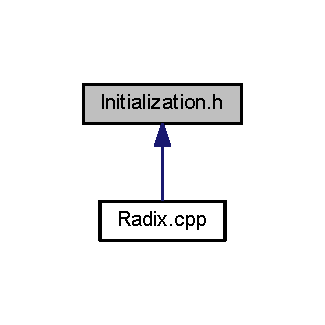
\includegraphics[width=156pt]{_initialization_8h__dep__incl}
\end{center}
\end{figure}
\subsection*{Функции}
\begin{DoxyCompactItemize}
\item 
void \hyperlink{_initialization_8h_a11b373fd61e18cd28810a5b607e1749a}{v\+\_\+initialization} ()
\end{DoxyCompactItemize}


\subsection{Подробное описание}
Заголовочный файл с вызовом модуля инициализации 

Вызов\+: 
\begin{DoxyCode}
\textcolor{keywordtype}{void} \hyperlink{_initialization_8cpp_a11b373fd61e18cd28810a5b607e1749a}{v\_initialization}();
\end{DoxyCode}


\begin{DoxyAuthor}{Автор}
Sava\+Lione 
\end{DoxyAuthor}


\subsection{Функции}
\mbox{\Hypertarget{_initialization_8h_a11b373fd61e18cd28810a5b607e1749a}\label{_initialization_8h_a11b373fd61e18cd28810a5b607e1749a}} 
\index{Initialization.\+h@{Initialization.\+h}!v\+\_\+initialization@{v\+\_\+initialization}}
\index{v\+\_\+initialization@{v\+\_\+initialization}!Initialization.\+h@{Initialization.\+h}}
\subsubsection{\texorpdfstring{v\+\_\+initialization()}{v\_initialization()}}
{\footnotesize\ttfamily void v\+\_\+initialization (\begin{DoxyParamCaption}{ }\end{DoxyParamCaption})}

Главная функция программы

Проверяет наличие 3 стандартных файлов программы \begin{DoxyVerb}logger.log

rules.txt

settings.ini\end{DoxyVerb}
 
\hypertarget{_ip_8cpp}{}\section{Файл Ip.\+cpp}
\label{_ip_8cpp}\index{Ip.\+cpp@{Ip.\+cpp}}


Модуль работы с ip адресами.  


{\ttfamily \#include $<$fstream$>$}\newline
{\ttfamily \#include $<$iostream$>$}\newline
{\ttfamily \#include $<$string$>$}\newline
{\ttfamily \#include \char`\"{}../core/\+Constants.\+h\char`\"{}}\newline
Граф включаемых заголовочных файлов для Ip.\+cpp\+:\nopagebreak
\begin{figure}[H]
\begin{center}
\leavevmode
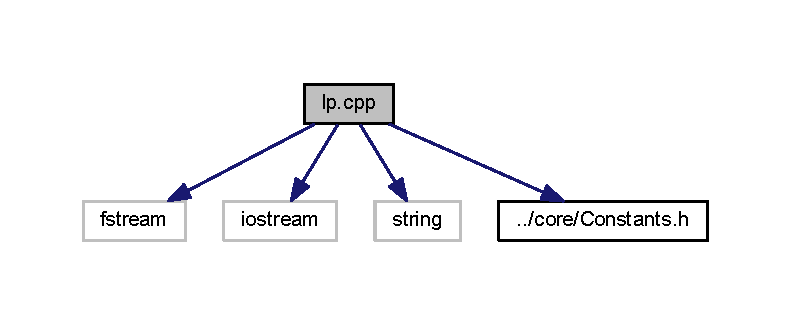
\includegraphics[width=350pt]{_ip_8cpp__incl}
\end{center}
\end{figure}
\subsection*{Функции}
\begin{DoxyCompactItemize}
\item 
void \hyperlink{_ip_8cpp_a456dd80d06da80bf51df048d22fae10c}{v\+\_\+convert\+\_\+ip} (char $\ast$ch\+\_\+ip\+\_\+addr, unsigned char $\ast$uc\+\_\+arr\+\_\+return)
\item 
void \hyperlink{_ip_8cpp_a8922c0342039e2f0d376c1d806eb84d2}{v\+\_\+get\+\_\+ip} (char $\ast$ch\+\_\+return)
\end{DoxyCompactItemize}


\subsection{Подробное описание}
Модуль работы с ip адресами. 

\begin{DoxyAuthor}{Автор}
Sava\+Lione 
\end{DoxyAuthor}


\subsection{Функции}
\mbox{\Hypertarget{_ip_8cpp_a456dd80d06da80bf51df048d22fae10c}\label{_ip_8cpp_a456dd80d06da80bf51df048d22fae10c}} 
\index{Ip.\+cpp@{Ip.\+cpp}!v\+\_\+convert\+\_\+ip@{v\+\_\+convert\+\_\+ip}}
\index{v\+\_\+convert\+\_\+ip@{v\+\_\+convert\+\_\+ip}!Ip.\+cpp@{Ip.\+cpp}}
\subsubsection{\texorpdfstring{v\+\_\+convert\+\_\+ip()}{v\_convert\_ip()}}
{\footnotesize\ttfamily void v\+\_\+convert\+\_\+ip (\begin{DoxyParamCaption}\item[{char $\ast$}]{ch\+\_\+ip\+\_\+addr,  }\item[{unsigned char $\ast$}]{uc\+\_\+arr\+\_\+return }\end{DoxyParamCaption})}

Парсинг ip адресов 
\begin{DoxyParams}[1]{Аргументы}
\mbox{\tt in}  & {\em ch\+\_\+ip\+\_\+addr} & Массив char с ip адресом \\
\hline
\mbox{\tt out}  & {\em uc\+\_\+arr\+\_\+return} & Возвращяет массив типа unsigned char \\
\hline
\end{DoxyParams}
\begin{DoxyReturn}{Возвращает}
Массив из 4 переменных типа unsigned char 
\end{DoxyReturn}
\begin{Desc}
\item[Примеры\+: ]\par
\hyperlink{v_convert_ip_8cpp-example}{v\+\_\+convert\+\_\+ip.\+cpp}.\end{Desc}
\mbox{\Hypertarget{_ip_8cpp_a8922c0342039e2f0d376c1d806eb84d2}\label{_ip_8cpp_a8922c0342039e2f0d376c1d806eb84d2}} 
\index{Ip.\+cpp@{Ip.\+cpp}!v\+\_\+get\+\_\+ip@{v\+\_\+get\+\_\+ip}}
\index{v\+\_\+get\+\_\+ip@{v\+\_\+get\+\_\+ip}!Ip.\+cpp@{Ip.\+cpp}}
\subsubsection{\texorpdfstring{v\+\_\+get\+\_\+ip()}{v\_get\_ip()}}
{\footnotesize\ttfamily void v\+\_\+get\+\_\+ip (\begin{DoxyParamCaption}\item[{char $\ast$}]{ch\+\_\+return }\end{DoxyParamCaption})}

Парсинг ip адресов 
\begin{DoxyParams}[1]{Аргументы}
\mbox{\tt out}  & {\em ch\+\_\+return} & Массив char, в который запишется ip адрес \\
\hline
\end{DoxyParams}
\begin{DoxyReturn}{Возвращает}
Массив символов, который запишется в ch\+\_\+return 
\end{DoxyReturn}
\begin{Desc}
\item[Примеры\+: ]\par
\hyperlink{v_get_ip_8cpp-example}{v\+\_\+get\+\_\+ip.\+cpp}.\end{Desc}

\hypertarget{_ip_8h}{}\section{Файл Ip.\+h}
\label{_ip_8h}\index{Ip.\+h@{Ip.\+h}}


Заголовочный файл с подключением модуля работы с ip адресами.  


Граф файлов, в которые включается этот файл\+:\nopagebreak
\begin{figure}[H]
\begin{center}
\leavevmode
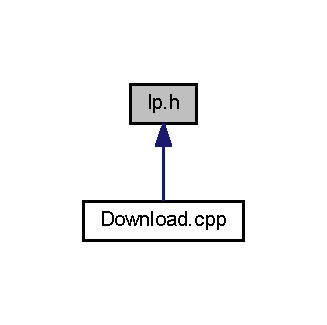
\includegraphics[width=157pt]{_ip_8h__dep__incl}
\end{center}
\end{figure}
\subsection*{Функции}
\begin{DoxyCompactItemize}
\item 
void \hyperlink{_ip_8h_a456dd80d06da80bf51df048d22fae10c}{v\+\_\+convert\+\_\+ip} (char $\ast$ch\+\_\+ip\+\_\+addr, unsigned char $\ast$uc\+\_\+arr\+\_\+return)
\item 
void \hyperlink{_ip_8h_a8922c0342039e2f0d376c1d806eb84d2}{v\+\_\+get\+\_\+ip} (char $\ast$ch\+\_\+return)
\end{DoxyCompactItemize}


\subsection{Подробное описание}
Заголовочный файл с подключением модуля работы с ip адресами. 

\begin{DoxyAuthor}{Автор}
Sava\+Lione 
\end{DoxyAuthor}


\subsection{Функции}
\mbox{\Hypertarget{_ip_8h_a456dd80d06da80bf51df048d22fae10c}\label{_ip_8h_a456dd80d06da80bf51df048d22fae10c}} 
\index{Ip.\+h@{Ip.\+h}!v\+\_\+convert\+\_\+ip@{v\+\_\+convert\+\_\+ip}}
\index{v\+\_\+convert\+\_\+ip@{v\+\_\+convert\+\_\+ip}!Ip.\+h@{Ip.\+h}}
\subsubsection{\texorpdfstring{v\+\_\+convert\+\_\+ip()}{v\_convert\_ip()}}
{\footnotesize\ttfamily void v\+\_\+convert\+\_\+ip (\begin{DoxyParamCaption}\item[{char $\ast$}]{ch\+\_\+ip\+\_\+addr,  }\item[{unsigned char $\ast$}]{uc\+\_\+arr\+\_\+return }\end{DoxyParamCaption})}

Парсинг ip адресов 
\begin{DoxyParams}[1]{Аргументы}
\mbox{\tt in}  & {\em ch\+\_\+ip\+\_\+addr} & Массив char с ip адресом \\
\hline
\mbox{\tt out}  & {\em uc\+\_\+arr\+\_\+return} & Возвращяет массив типа unsigned char \\
\hline
\end{DoxyParams}
\begin{DoxyReturn}{Возвращает}
Массив из 4 переменных типа unsigned char 
\end{DoxyReturn}
\mbox{\Hypertarget{_ip_8h_a8922c0342039e2f0d376c1d806eb84d2}\label{_ip_8h_a8922c0342039e2f0d376c1d806eb84d2}} 
\index{Ip.\+h@{Ip.\+h}!v\+\_\+get\+\_\+ip@{v\+\_\+get\+\_\+ip}}
\index{v\+\_\+get\+\_\+ip@{v\+\_\+get\+\_\+ip}!Ip.\+h@{Ip.\+h}}
\subsubsection{\texorpdfstring{v\+\_\+get\+\_\+ip()}{v\_get\_ip()}}
{\footnotesize\ttfamily void v\+\_\+get\+\_\+ip (\begin{DoxyParamCaption}\item[{char $\ast$}]{ch\+\_\+return }\end{DoxyParamCaption})}

Парсинг ip адресов 
\begin{DoxyParams}[1]{Аргументы}
\mbox{\tt out}  & {\em ch\+\_\+return} & Массив char, в который запишется ip адрес \\
\hline
\end{DoxyParams}
\begin{DoxyReturn}{Возвращает}
Массив символов, который запишется в ch\+\_\+return 
\end{DoxyReturn}

\hypertarget{_logger_8cpp}{}\section{Файл Logger.\+cpp}
\label{_logger_8cpp}\index{Logger.\+cpp@{Logger.\+cpp}}


Модуль логирования  


{\ttfamily \#include $<$string$>$}\newline
{\ttfamily \#include $<$fstream$>$}\newline
{\ttfamily \#include $<$thread$>$}\newline
{\ttfamily \#include $<$windows.\+h$>$}\newline
{\ttfamily \#include $<$stdio.\+h$>$}\newline
{\ttfamily \#include \char`\"{}Logger.\+h\char`\"{}}\newline
{\ttfamily \#include \char`\"{}Settings.\+h\char`\"{}}\newline
Граф включаемых заголовочных файлов для Logger.\+cpp\+:\nopagebreak
\begin{figure}[H]
\begin{center}
\leavevmode
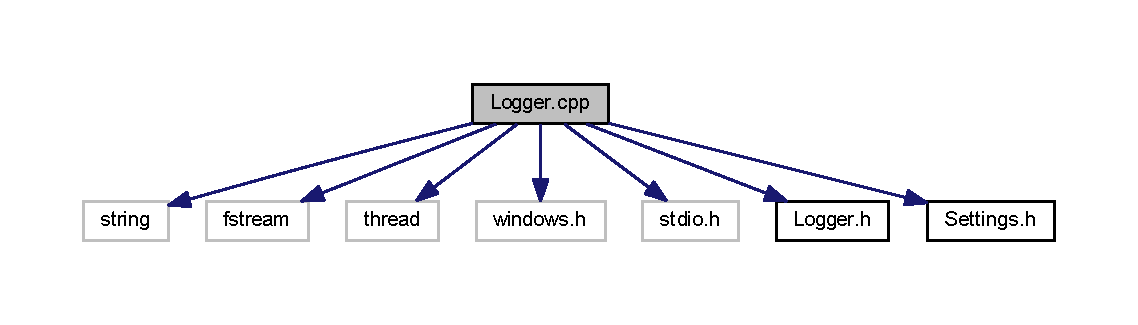
\includegraphics[width=350pt]{_logger_8cpp__incl}
\end{center}
\end{figure}
\subsection*{Функции}
\begin{DoxyCompactItemize}
\item 
void \hyperlink{_logger_8cpp_a37ded7634d8547536bbd135208109766}{log\+\_\+thr} (string \&s, string \&level)
\item 
void \hyperlink{_logger_8cpp_a85cbef1702d055318336f0f3a5036959}{log} (string level, string s)
\end{DoxyCompactItemize}


\subsection{Подробное описание}
Модуль логирования 


\begin{DoxyCode}
Логгер
Логгирование сообщений в файл logger.log
Уровеней лога - 3
Уровень 0:
Вывод сообщений вида:
    [                   ] \{MESSAGE\}
Применение:
    Обработка простых сообщений, без времени и префикса ([PREFIX])
Уровень 1:
Вывод сообщений вида:
    [\{YEAR\}/\{MONTH\}/\{DAY\} \{HOUR\}:\{MINUTE\}:\{SECOND\}] [LOG] \{MESSAGE\}
Применение:
    Обработка простых сообщений(загрузка модуля, отключение модуля, вход в программу, выход из программы и 
      тд.) С временем и префиксом ([LOG])
Уровень 2:
Вывод сообщений вида:
    [\{YEAR\}/\{MONTH\}/\{DAY\} \{HOUR\}:\{MINUTE\}:\{SECOND\}] [WARN] \{MESSAGE\}
Применение:
    Обработка важных сообщений ошибки(не удачная загрузка модуля, не удачный вход в программу, экстренный 
      выход из программы и тд.) С временем и префиксом ([WARN])
\end{DoxyCode}


\begin{DoxyAuthor}{Автор}
Sava\+Lione 
\end{DoxyAuthor}


\subsection{Функции}
\mbox{\Hypertarget{_logger_8cpp_a85cbef1702d055318336f0f3a5036959}\label{_logger_8cpp_a85cbef1702d055318336f0f3a5036959}} 
\index{Logger.\+cpp@{Logger.\+cpp}!log@{log}}
\index{log@{log}!Logger.\+cpp@{Logger.\+cpp}}
\subsubsection{\texorpdfstring{log()}{log()}}
{\footnotesize\ttfamily void log (\begin{DoxyParamCaption}\item[{string}]{level,  }\item[{string}]{s }\end{DoxyParamCaption})}

Логгирование сообщений в файл logger.\+log 
\begin{DoxyParams}[1]{Аргументы}
\mbox{\tt in}  & {\em level} & Уровень логирования \\
\hline
\mbox{\tt in}  & {\em s} & Логируемая информация \\
\hline
\end{DoxyParams}
\mbox{\Hypertarget{_logger_8cpp_a37ded7634d8547536bbd135208109766}\label{_logger_8cpp_a37ded7634d8547536bbd135208109766}} 
\index{Logger.\+cpp@{Logger.\+cpp}!log\+\_\+thr@{log\+\_\+thr}}
\index{log\+\_\+thr@{log\+\_\+thr}!Logger.\+cpp@{Logger.\+cpp}}
\subsubsection{\texorpdfstring{log\+\_\+thr()}{log\_thr()}}
{\footnotesize\ttfamily void log\+\_\+thr (\begin{DoxyParamCaption}\item[{string \&}]{s,  }\item[{string \&}]{level }\end{DoxyParamCaption})}

Функция, для записи лога в файл 
\begin{DoxyParams}[1]{Аргументы}
\mbox{\tt in}  & {\em \&s} & Передача ссылки с сообщением для логирования \\
\hline
\mbox{\tt in}  & {\em \&level} & Передача ссылки с уровнем логирования \\
\hline
\end{DoxyParams}

\hypertarget{_logger_8h}{}\section{Файл Logger.\+h}
\label{_logger_8h}\index{Logger.\+h@{Logger.\+h}}


Заголовочный файл с подключением модуля логирования.  


{\ttfamily \#include $<$string$>$}\newline
Граф включаемых заголовочных файлов для Logger.\+h\+:\nopagebreak
\begin{figure}[H]
\begin{center}
\leavevmode
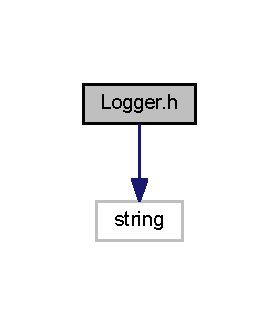
\includegraphics[width=134pt]{_logger_8h__incl}
\end{center}
\end{figure}
Граф файлов, в которые включается этот файл\+:\nopagebreak
\begin{figure}[H]
\begin{center}
\leavevmode
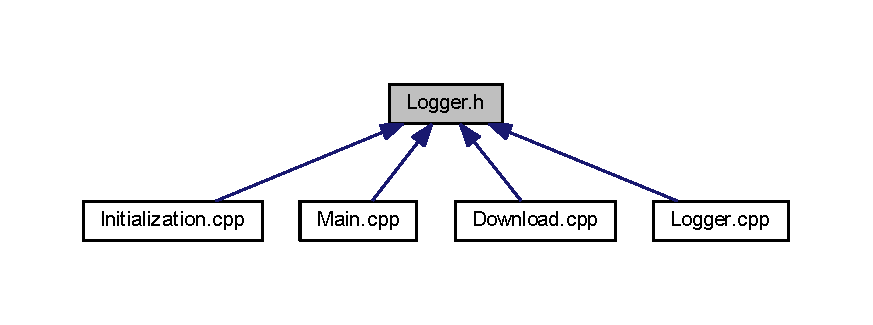
\includegraphics[width=350pt]{_logger_8h__dep__incl}
\end{center}
\end{figure}
\subsection*{Функции}
\begin{DoxyCompactItemize}
\item 
void \hyperlink{_logger_8h_ad35770e66782b0d5c63307682c5de765}{log} (std\+::string level, std\+::string s)
\end{DoxyCompactItemize}


\subsection{Подробное описание}
Заголовочный файл с подключением модуля логирования. 

\begin{DoxyAuthor}{Автор}
Sava\+Lione 
\end{DoxyAuthor}


\subsection{Функции}
\mbox{\Hypertarget{_logger_8h_ad35770e66782b0d5c63307682c5de765}\label{_logger_8h_ad35770e66782b0d5c63307682c5de765}} 
\index{Logger.\+h@{Logger.\+h}!log@{log}}
\index{log@{log}!Logger.\+h@{Logger.\+h}}
\subsubsection{\texorpdfstring{log()}{log()}}
{\footnotesize\ttfamily void log (\begin{DoxyParamCaption}\item[{std\+::string}]{level,  }\item[{std\+::string}]{s }\end{DoxyParamCaption})}

Логгирование сообщений в файл logger.\+log 
\begin{DoxyParams}[1]{Аргументы}
\mbox{\tt in}  & {\em level} & Уровень логирования \\
\hline
\mbox{\tt in}  & {\em s} & Логируемая информация \\
\hline
\end{DoxyParams}

\hypertarget{_main_8cpp}{}\section{Файл Main.\+cpp}
\label{_main_8cpp}\index{Main.\+cpp@{Main.\+cpp}}


Главный файл программы  


{\ttfamily \#include $<$Windows.\+h$>$}\newline
{\ttfamily \#include $<$iostream$>$}\newline
{\ttfamily \#include $<$cstring$>$}\newline
{\ttfamily \#include $<$string$>$}\newline
{\ttfamily \#include \char`\"{}..\textbackslash{}io\textbackslash{}\+Settings.\+h\char`\"{}}\newline
{\ttfamily \#include \char`\"{}Radix.\+h\char`\"{}}\newline
{\ttfamily \#include \char`\"{}..\textbackslash{}io\textbackslash{}\+Logger.\+h\char`\"{}}\newline
Граф включаемых заголовочных файлов для Main.\+cpp\+:
\nopagebreak
\begin{figure}[H]
\begin{center}
\leavevmode
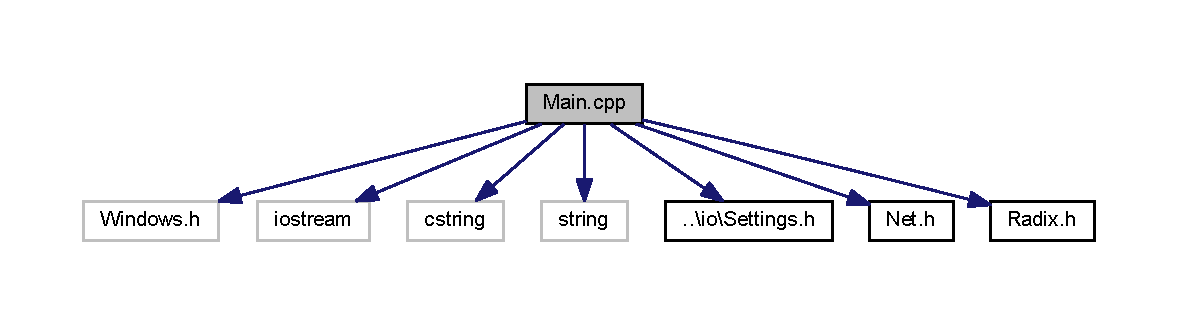
\includegraphics[width=350pt]{_main_8cpp__incl}
\end{center}
\end{figure}
\subsection*{Функции}
\begin{DoxyCompactItemize}
\item 
int \hyperlink{_main_8cpp_ae66f6b31b5ad750f1fe042a706a4e3d4}{main} ()
\end{DoxyCompactItemize}


\subsection{Подробное описание}
Главный файл программы 

\begin{DoxyAuthor}{Автор}
Sava\+Lione 
\end{DoxyAuthor}


\subsection{Функции}
\mbox{\Hypertarget{_main_8cpp_ae66f6b31b5ad750f1fe042a706a4e3d4}\label{_main_8cpp_ae66f6b31b5ad750f1fe042a706a4e3d4}} 
\index{Main.\+cpp@{Main.\+cpp}!main@{main}}
\index{main@{main}!Main.\+cpp@{Main.\+cpp}}
\subsubsection{\texorpdfstring{main()}{main()}}
{\footnotesize\ttfamily int main (\begin{DoxyParamCaption}{ }\end{DoxyParamCaption})}

\begin{DoxyReturn}{Возвращает}
Код завершения программы Вызов программы компилятором 
\end{DoxyReturn}
$<$ Запуск программы 



$<$ Пауза до нажатия любой клавиши 

\begin{Desc}
\item[Примеры\+: ]\par
\hyperlink{log_8cpp-example}{log.\+cpp}.\end{Desc}


См. определение в файле Main.\+cpp строка 23


\hypertarget{_radix_8cpp}{}\section{Файл Radix.\+cpp}
\label{_radix_8cpp}\index{Radix.\+cpp@{Radix.\+cpp}}


Главный файл программы  


{\ttfamily \#include \char`\"{}Initialization.\+h\char`\"{}}\newline
Граф включаемых заголовочных файлов для Radix.\+cpp\+:\nopagebreak
\begin{figure}[H]
\begin{center}
\leavevmode
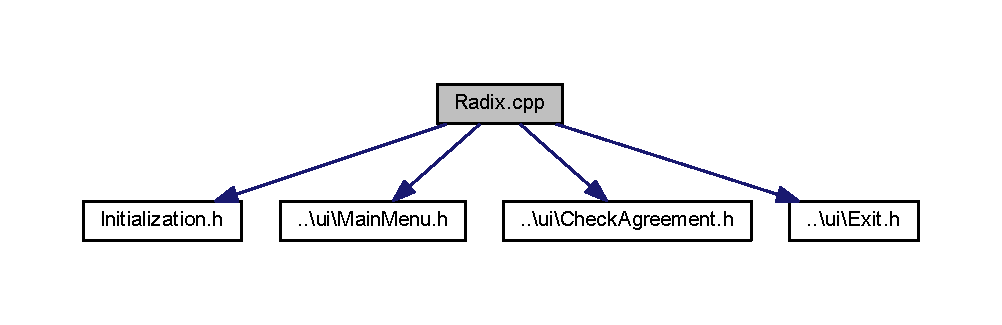
\includegraphics[width=156pt]{_radix_8cpp__incl}
\end{center}
\end{figure}
\subsection*{Функции}
\begin{DoxyCompactItemize}
\item 
void \hyperlink{_radix_8cpp_a86a56c401ce2783ee9288b33af746520}{Radix} ()
\begin{DoxyCompactList}\small\item\em Запуск программы \end{DoxyCompactList}\end{DoxyCompactItemize}


\subsection{Подробное описание}
Главный файл программы 

\begin{DoxyAuthor}{Автор}
Sava\+Lione 
\end{DoxyAuthor}


\subsection{Функции}
\mbox{\Hypertarget{_radix_8cpp_a86a56c401ce2783ee9288b33af746520}\label{_radix_8cpp_a86a56c401ce2783ee9288b33af746520}} 
\index{Radix.\+cpp@{Radix.\+cpp}!Radix@{Radix}}
\index{Radix@{Radix}!Radix.\+cpp@{Radix.\+cpp}}
\subsubsection{\texorpdfstring{Radix()}{Radix()}}
{\footnotesize\ttfamily void Radix (\begin{DoxyParamCaption}{ }\end{DoxyParamCaption})}



Запуск программы 

Запуск модуля инициализации 
\hypertarget{_radix_8h}{}\section{Файл Radix.\+h}
\label{_radix_8h}\index{Radix.\+h@{Radix.\+h}}


Заголовочный файл с вызовом главной функции программы  


Граф файлов, в которые включается этот файл\+:
\nopagebreak
\begin{figure}[H]
\begin{center}
\leavevmode
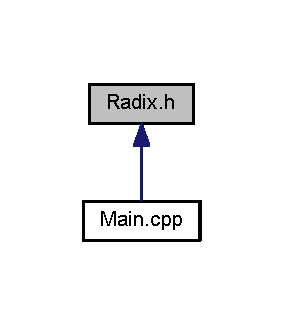
\includegraphics[width=136pt]{d6/db2/_radix_8h__dep__incl}
\end{center}
\end{figure}
\subsection*{Функции}
\begin{DoxyCompactItemize}
\item 
void \hyperlink{_radix_8h_a86a56c401ce2783ee9288b33af746520}{Radix} ()
\begin{DoxyCompactList}\small\item\em Запуск программы \end{DoxyCompactList}\end{DoxyCompactItemize}


\subsection{Подробное описание}
Заголовочный файл с вызовом главной функции программы 

\begin{DoxyAuthor}{Автор}
Sava\+Lione 
\end{DoxyAuthor}


\subsection{Функции}
\mbox{\Hypertarget{_radix_8h_a86a56c401ce2783ee9288b33af746520}\label{_radix_8h_a86a56c401ce2783ee9288b33af746520}} 
\index{Radix.\+h@{Radix.\+h}!Radix@{Radix}}
\index{Radix@{Radix}!Radix.\+h@{Radix.\+h}}
\subsubsection{\texorpdfstring{Radix()}{Radix()}}
{\footnotesize\ttfamily void Radix (\begin{DoxyParamCaption}{ }\end{DoxyParamCaption})}



Запуск программы 

$<$ Запуск модуля инициализации 
\hypertarget{_settings_8cpp}{}\section{Файл Settings.\+cpp}
\label{_settings_8cpp}\index{Settings.\+cpp@{Settings.\+cpp}}


Модуль настроек. Парсит переменные в файлах  


{\ttfamily \#include $<$fstream$>$}\newline
{\ttfamily \#include $<$string$>$}\newline
{\ttfamily \#include \char`\"{}../core/\+Constants.\+h\char`\"{}}\newline
Граф включаемых заголовочных файлов для Settings.\+cpp\+:\nopagebreak
\begin{figure}[H]
\begin{center}
\leavevmode
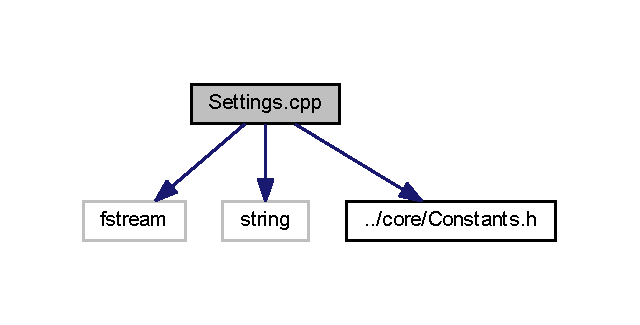
\includegraphics[width=307pt]{_settings_8cpp__incl}
\end{center}
\end{figure}
\subsection*{Функции}
\begin{DoxyCompactItemize}
\item 
bool \hyperlink{_settings_8cpp_a7fcd42142e325cb27a380f49d655f9de}{b\+\_\+settings} (char ch\+\_\+arr\+\_\+value\mbox{[}$\,$\mbox{]})
\end{DoxyCompactItemize}


\subsection{Подробное описание}
Модуль настроек. Парсит переменные в файлах 

\begin{DoxyAuthor}{Автор}
Sava\+Lione 
\end{DoxyAuthor}


\subsection{Функции}
\mbox{\Hypertarget{_settings_8cpp_a7fcd42142e325cb27a380f49d655f9de}\label{_settings_8cpp_a7fcd42142e325cb27a380f49d655f9de}} 
\index{Settings.\+cpp@{Settings.\+cpp}!b\+\_\+settings@{b\+\_\+settings}}
\index{b\+\_\+settings@{b\+\_\+settings}!Settings.\+cpp@{Settings.\+cpp}}
\subsubsection{\texorpdfstring{b\+\_\+settings()}{b\_settings()}}
{\footnotesize\ttfamily bool b\+\_\+settings (\begin{DoxyParamCaption}\item[{char}]{ch\+\_\+arr\+\_\+value\mbox{[}$\,$\mbox{]} }\end{DoxyParamCaption})}

Парсинг параметров 
\begin{DoxyParams}[1]{Аргументы}
\mbox{\tt in}  & {\em ch\+\_\+arr\+\_\+value\mbox{[}$\,$\mbox{]}} & Значение, которое надо найти в файле \\
\hline
\end{DoxyParams}
\begin{DoxyReturn}{Возвращает}
Значение переменной true false 
\end{DoxyReturn}

\hypertarget{_settings_8h}{}\section{Файл Settings.\+h}
\label{_settings_8h}\index{Settings.\+h@{Settings.\+h}}


Заголовочный файл с подключением модуля настроек.  


Граф файлов, в которые включается этот файл\+:\nopagebreak
\begin{figure}[H]
\begin{center}
\leavevmode
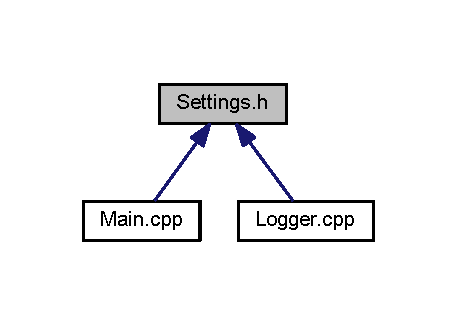
\includegraphics[width=220pt]{_settings_8h__dep__incl}
\end{center}
\end{figure}
\subsection*{Функции}
\begin{DoxyCompactItemize}
\item 
bool \hyperlink{_settings_8h_a7fcd42142e325cb27a380f49d655f9de}{b\+\_\+settings} (char ch\+\_\+arr\+\_\+value\mbox{[}$\,$\mbox{]})
\item 
void \hyperlink{_settings_8h_a8922c0342039e2f0d376c1d806eb84d2}{v\+\_\+get\+\_\+ip} (char $\ast$ch\+\_\+return)
\end{DoxyCompactItemize}


\subsection{Подробное описание}
Заголовочный файл с подключением модуля настроек. 

\begin{DoxyAuthor}{Автор}
Sava\+Lione 
\end{DoxyAuthor}


\subsection{Функции}
\mbox{\Hypertarget{_settings_8h_a7fcd42142e325cb27a380f49d655f9de}\label{_settings_8h_a7fcd42142e325cb27a380f49d655f9de}} 
\index{Settings.\+h@{Settings.\+h}!b\+\_\+settings@{b\+\_\+settings}}
\index{b\+\_\+settings@{b\+\_\+settings}!Settings.\+h@{Settings.\+h}}
\subsubsection{\texorpdfstring{b\+\_\+settings()}{b\_settings()}}
{\footnotesize\ttfamily bool b\+\_\+settings (\begin{DoxyParamCaption}\item[{char}]{ch\+\_\+arr\+\_\+value\mbox{[}$\,$\mbox{]} }\end{DoxyParamCaption})}

Парсинг параметров 
\begin{DoxyParams}[1]{Аргументы}
\mbox{\tt in}  & {\em ch\+\_\+arr\+\_\+value\mbox{[}$\,$\mbox{]}} & Значение, которое надо найти в файле \\
\hline
\end{DoxyParams}
\begin{DoxyReturn}{Возвращает}
Значение переменной true false 
\end{DoxyReturn}
\mbox{\Hypertarget{_settings_8h_a8922c0342039e2f0d376c1d806eb84d2}\label{_settings_8h_a8922c0342039e2f0d376c1d806eb84d2}} 
\index{Settings.\+h@{Settings.\+h}!v\+\_\+get\+\_\+ip@{v\+\_\+get\+\_\+ip}}
\index{v\+\_\+get\+\_\+ip@{v\+\_\+get\+\_\+ip}!Settings.\+h@{Settings.\+h}}
\subsubsection{\texorpdfstring{v\+\_\+get\+\_\+ip()}{v\_get\_ip()}}
{\footnotesize\ttfamily void v\+\_\+get\+\_\+ip (\begin{DoxyParamCaption}\item[{char $\ast$}]{ch\+\_\+return }\end{DoxyParamCaption})}

Парсинг ip адресов 
\begin{DoxyParams}[1]{Аргументы}
\mbox{\tt out}  & {\em ch\+\_\+return} & Массив char, в который запишется ip адрес \\
\hline
\end{DoxyParams}
\begin{DoxyReturn}{Возвращает}
Массив символов, который запишется в ch\+\_\+return 
\end{DoxyReturn}

\hypertarget{_templates_8cpp}{}\section{Файл Templates.\+cpp}
\label{_templates_8cpp}\index{Templates.\+cpp@{Templates.\+cpp}}


Функции для создания стандартных файлов программы.  


{\ttfamily \#include $<$fstream$>$}\newline
{\ttfamily \#include \char`\"{}Templates.\+h\char`\"{}}\newline
{\ttfamily \#include \char`\"{}..\textbackslash{}core\textbackslash{}\+Constants.\+h\char`\"{}}\newline
Граф включаемых заголовочных файлов для Templates.\+cpp\+:
\nopagebreak
\begin{figure}[H]
\begin{center}
\leavevmode
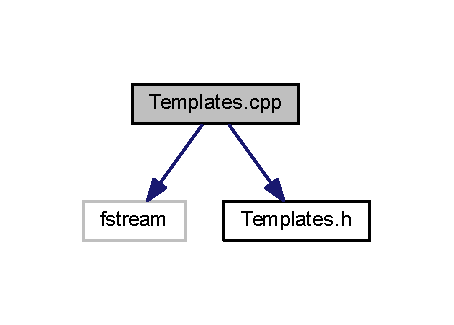
\includegraphics[width=336pt]{_templates_8cpp__incl}
\end{center}
\end{figure}
\subsection*{Функции}
\begin{DoxyCompactItemize}
\item 
void \hyperlink{_templates_8cpp_abeb0b4d4d31b9c74744a0b9881d95066}{v\+\_\+templates\+\_\+create\+\_\+logger\+\_\+log} ()
\item 
void \hyperlink{_templates_8cpp_afbd4b91587b894d5e8b6ea50209ed5dc}{v\+\_\+templates\+\_\+create\+\_\+rules\+\_\+txt} ()
\item 
void \hyperlink{_templates_8cpp_a593e33d5988d6a49d581f52d94471895}{v\+\_\+templates\+\_\+create\+\_\+settings\+\_\+ini} ()
\item 
void \hyperlink{_templates_8cpp_a4cdca62a0922d9ad016c50f1251636cb}{v\+\_\+templates\+\_\+create\+\_\+ip\+\_\+ini} ()
\end{DoxyCompactItemize}


\subsection{Подробное описание}
Функции для создания стандартных файлов программы. 

\begin{DoxyAuthor}{Автор}
Sava\+Lione 
\end{DoxyAuthor}


\subsection{Функции}
\mbox{\Hypertarget{_templates_8cpp_a4cdca62a0922d9ad016c50f1251636cb}\label{_templates_8cpp_a4cdca62a0922d9ad016c50f1251636cb}} 
\index{Templates.\+cpp@{Templates.\+cpp}!v\+\_\+templates\+\_\+create\+\_\+ip\+\_\+ini@{v\+\_\+templates\+\_\+create\+\_\+ip\+\_\+ini}}
\index{v\+\_\+templates\+\_\+create\+\_\+ip\+\_\+ini@{v\+\_\+templates\+\_\+create\+\_\+ip\+\_\+ini}!Templates.\+cpp@{Templates.\+cpp}}
\subsubsection{\texorpdfstring{v\+\_\+templates\+\_\+create\+\_\+ip\+\_\+ini()}{v\_templates\_create\_ip\_ini()}}
{\footnotesize\ttfamily void v\+\_\+templates\+\_\+create\+\_\+ip\+\_\+ini (\begin{DoxyParamCaption}{ }\end{DoxyParamCaption})}

Создание файла ip. \begin{DoxyVerb}ip.ini - файл с ip адресами\end{DoxyVerb}
 

См. определение в файле Templates.\+cpp строка 83

\mbox{\Hypertarget{_templates_8cpp_abeb0b4d4d31b9c74744a0b9881d95066}\label{_templates_8cpp_abeb0b4d4d31b9c74744a0b9881d95066}} 
\index{Templates.\+cpp@{Templates.\+cpp}!v\+\_\+templates\+\_\+create\+\_\+logger\+\_\+log@{v\+\_\+templates\+\_\+create\+\_\+logger\+\_\+log}}
\index{v\+\_\+templates\+\_\+create\+\_\+logger\+\_\+log@{v\+\_\+templates\+\_\+create\+\_\+logger\+\_\+log}!Templates.\+cpp@{Templates.\+cpp}}
\subsubsection{\texorpdfstring{v\+\_\+templates\+\_\+create\+\_\+logger\+\_\+log()}{v\_templates\_create\_logger\_log()}}
{\footnotesize\ttfamily void v\+\_\+templates\+\_\+create\+\_\+logger\+\_\+log (\begin{DoxyParamCaption}{ }\end{DoxyParamCaption})}

Создание файла пользовательского соглашения. \begin{DoxyVerb}logger.log - файл с логом вывода\end{DoxyVerb}
 

См. определение в файле Templates.\+cpp строка 21

\mbox{\Hypertarget{_templates_8cpp_afbd4b91587b894d5e8b6ea50209ed5dc}\label{_templates_8cpp_afbd4b91587b894d5e8b6ea50209ed5dc}} 
\index{Templates.\+cpp@{Templates.\+cpp}!v\+\_\+templates\+\_\+create\+\_\+rules\+\_\+txt@{v\+\_\+templates\+\_\+create\+\_\+rules\+\_\+txt}}
\index{v\+\_\+templates\+\_\+create\+\_\+rules\+\_\+txt@{v\+\_\+templates\+\_\+create\+\_\+rules\+\_\+txt}!Templates.\+cpp@{Templates.\+cpp}}
\subsubsection{\texorpdfstring{v\+\_\+templates\+\_\+create\+\_\+rules\+\_\+txt()}{v\_templates\_create\_rules\_txt()}}
{\footnotesize\ttfamily void v\+\_\+templates\+\_\+create\+\_\+rules\+\_\+txt (\begin{DoxyParamCaption}{ }\end{DoxyParamCaption})}

Создание файла пользовательского соглашения. \begin{DoxyVerb}rules.txt - файл с пользовательским соглашением\end{DoxyVerb}
 

См. определение в файле Templates.\+cpp строка 38

\mbox{\Hypertarget{_templates_8cpp_a593e33d5988d6a49d581f52d94471895}\label{_templates_8cpp_a593e33d5988d6a49d581f52d94471895}} 
\index{Templates.\+cpp@{Templates.\+cpp}!v\+\_\+templates\+\_\+create\+\_\+settings\+\_\+ini@{v\+\_\+templates\+\_\+create\+\_\+settings\+\_\+ini}}
\index{v\+\_\+templates\+\_\+create\+\_\+settings\+\_\+ini@{v\+\_\+templates\+\_\+create\+\_\+settings\+\_\+ini}!Templates.\+cpp@{Templates.\+cpp}}
\subsubsection{\texorpdfstring{v\+\_\+templates\+\_\+create\+\_\+settings\+\_\+ini()}{v\_templates\_create\_settings\_ini()}}
{\footnotesize\ttfamily void v\+\_\+templates\+\_\+create\+\_\+settings\+\_\+ini (\begin{DoxyParamCaption}{ }\end{DoxyParamCaption})}

Создание файла настроек. \begin{DoxyVerb}settings.ini - файл с настройками\end{DoxyVerb}
 

См. определение в файле Templates.\+cpp строка 59


\hypertarget{_templates_8h}{}\section{Файл Templates.\+h}
\label{_templates_8h}\index{Templates.\+h@{Templates.\+h}}


Заголовочный файл с подключением модуля создания стандартных файлов программы.  


Граф файлов, в которые включается этот файл\+:
\nopagebreak
\begin{figure}[H]
\begin{center}
\leavevmode
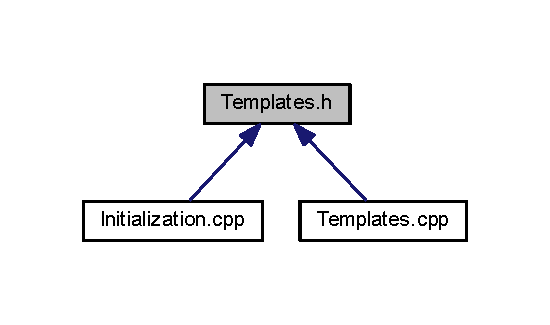
\includegraphics[width=264pt]{_templates_8h__dep__incl}
\end{center}
\end{figure}
\subsection*{Функции}
\begin{DoxyCompactItemize}
\item 
void \hyperlink{_templates_8h_abeb0b4d4d31b9c74744a0b9881d95066}{v\+\_\+templates\+\_\+create\+\_\+logger\+\_\+log} ()
\item 
void \hyperlink{_templates_8h_afbd4b91587b894d5e8b6ea50209ed5dc}{v\+\_\+templates\+\_\+create\+\_\+rules\+\_\+txt} ()
\item 
void \hyperlink{_templates_8h_a593e33d5988d6a49d581f52d94471895}{v\+\_\+templates\+\_\+create\+\_\+settings\+\_\+ini} ()
\end{DoxyCompactItemize}


\subsection{Подробное описание}
Заголовочный файл с подключением модуля создания стандартных файлов программы. 

\begin{DoxyAuthor}{Автор}
Sava\+Lione 
\end{DoxyAuthor}


\subsection{Функции}
\mbox{\Hypertarget{_templates_8h_abeb0b4d4d31b9c74744a0b9881d95066}\label{_templates_8h_abeb0b4d4d31b9c74744a0b9881d95066}} 
\index{Templates.\+h@{Templates.\+h}!v\+\_\+templates\+\_\+create\+\_\+logger\+\_\+log@{v\+\_\+templates\+\_\+create\+\_\+logger\+\_\+log}}
\index{v\+\_\+templates\+\_\+create\+\_\+logger\+\_\+log@{v\+\_\+templates\+\_\+create\+\_\+logger\+\_\+log}!Templates.\+h@{Templates.\+h}}
\subsubsection{\texorpdfstring{v\+\_\+templates\+\_\+create\+\_\+logger\+\_\+log()}{v\_templates\_create\_logger\_log()}}
{\footnotesize\ttfamily void v\+\_\+templates\+\_\+create\+\_\+logger\+\_\+log (\begin{DoxyParamCaption}{ }\end{DoxyParamCaption})}

Создание файла пользовательского соглашения. \begin{DoxyVerb}logger.log - файл с логом вывода\end{DoxyVerb}
 

См. определение в файле Templates.\+cpp строка 21

\mbox{\Hypertarget{_templates_8h_afbd4b91587b894d5e8b6ea50209ed5dc}\label{_templates_8h_afbd4b91587b894d5e8b6ea50209ed5dc}} 
\index{Templates.\+h@{Templates.\+h}!v\+\_\+templates\+\_\+create\+\_\+rules\+\_\+txt@{v\+\_\+templates\+\_\+create\+\_\+rules\+\_\+txt}}
\index{v\+\_\+templates\+\_\+create\+\_\+rules\+\_\+txt@{v\+\_\+templates\+\_\+create\+\_\+rules\+\_\+txt}!Templates.\+h@{Templates.\+h}}
\subsubsection{\texorpdfstring{v\+\_\+templates\+\_\+create\+\_\+rules\+\_\+txt()}{v\_templates\_create\_rules\_txt()}}
{\footnotesize\ttfamily void v\+\_\+templates\+\_\+create\+\_\+rules\+\_\+txt (\begin{DoxyParamCaption}{ }\end{DoxyParamCaption})}

Создание файла пользовательского соглашения. \begin{DoxyVerb}rules.txt - файл с пользовательским соглашением\end{DoxyVerb}
 

См. определение в файле Templates.\+cpp строка 38

\mbox{\Hypertarget{_templates_8h_a593e33d5988d6a49d581f52d94471895}\label{_templates_8h_a593e33d5988d6a49d581f52d94471895}} 
\index{Templates.\+h@{Templates.\+h}!v\+\_\+templates\+\_\+create\+\_\+settings\+\_\+ini@{v\+\_\+templates\+\_\+create\+\_\+settings\+\_\+ini}}
\index{v\+\_\+templates\+\_\+create\+\_\+settings\+\_\+ini@{v\+\_\+templates\+\_\+create\+\_\+settings\+\_\+ini}!Templates.\+h@{Templates.\+h}}
\subsubsection{\texorpdfstring{v\+\_\+templates\+\_\+create\+\_\+settings\+\_\+ini()}{v\_templates\_create\_settings\_ini()}}
{\footnotesize\ttfamily void v\+\_\+templates\+\_\+create\+\_\+settings\+\_\+ini (\begin{DoxyParamCaption}{ }\end{DoxyParamCaption})}

Создание файла настроек. \begin{DoxyVerb}settings.ini - файл с настройками\end{DoxyVerb}
 

См. определение в файле Templates.\+cpp строка 59


\chapter{Примеры}
\hypertarget{log_8cpp-example}{}\section{log.\+cpp}
\begin{DoxyAuthor}{Автор}
Sava\+Lione
\end{DoxyAuthor}

\begin{DoxyCodeInclude}
\textcolor{preprocessor}{#include "..\(\backslash\)io\(\backslash\)Logger.h"}

\textcolor{keywordtype}{int} \hyperlink{_main_8cpp_ae66f6b31b5ad750f1fe042a706a4e3d4}{main}() \{
    \hyperlink{_logger_8cpp_a85cbef1702d055318336f0f3a5036959}{log}(\textcolor{stringliteral}{"LOG"}, \textcolor{stringliteral}{"Hello World!!!"});
    \textcolor{keywordflow}{return} 0;
\}
\end{DoxyCodeInclude}
 
\hypertarget{v_convert_ip_8cpp-example}{}\section{v\+\_\+convert\+\_\+ip.\+cpp}
Парсинг ip адресов 
\begin{DoxyParams}[1]{Аргументы}
\mbox{\tt in}  & {\em ch\+\_\+ip\+\_\+addr} & Массив char с ip адресом \\
\hline
\mbox{\tt out}  & {\em uc\+\_\+arr\+\_\+return} & Возвращяет массив типа unsigned char \\
\hline
\end{DoxyParams}
\begin{DoxyReturn}{Возвращает}
Массив из 4 переменных типа unsigned char
\end{DoxyReturn}

\begin{DoxyCodeInclude}
\textcolor{preprocessor}{#include "..\(\backslash\)io\(\backslash\)Ip.h"}

\textcolor{keywordtype}{int} \hyperlink{_main_8cpp_ae66f6b31b5ad750f1fe042a706a4e3d4}{main}() \{
    \textcolor{keywordtype}{unsigned} \textcolor{keywordtype}{char} uc\_arr[4];
    \textcolor{keywordtype}{char} ch\_ip\_addr[16] = \textcolor{stringliteral}{"172.1.1.1"};
    \hyperlink{_ip_8cpp_a456dd80d06da80bf51df048d22fae10c}{v\_convert\_ip}(ch\_ip\_addr, uc\_arr);
    \textcolor{keywordflow}{return} 0;
\}
\end{DoxyCodeInclude}
 
\hypertarget{v_download_file_8cpp-example}{}\section{v\+\_\+download\+\_\+file.\+cpp}
Загрузка файла по уникальному номеру 
\begin{DoxyParams}[1]{Аргументы}
\mbox{\tt in}  & {\em sz\+\_\+file} & Номер файла для загрузки\\
\hline
\end{DoxyParams}

\begin{DoxyCodeInclude}
\textcolor{preprocessor}{#include "..\(\backslash\)io\(\backslash\)Download.h"}

\textcolor{keywordtype}{int} \hyperlink{_main_8cpp_ae66f6b31b5ad750f1fe042a706a4e3d4}{main}() \{
    \textcolor{keywordtype}{size\_t} sz\_file = 0123;
    \hyperlink{_download_8cpp_ab3291bd9df2e78c286f024fb1df3a683}{v\_download\_file}(sz\_file);
    \textcolor{keywordflow}{return} 0;
\}
\end{DoxyCodeInclude}
 
\hypertarget{v_get_ip_8cpp-example}{}\section{v\+\_\+get\+\_\+ip.\+cpp}
Парсинг ip адресов 
\begin{DoxyParams}[1]{Аргументы}
\mbox{\tt out}  & {\em ch\+\_\+return} & Массив char, в который запишется ip адрес \\
\hline
\end{DoxyParams}
\begin{DoxyReturn}{Возвращает}
Массив символов, который запишется в ch\+\_\+return
\end{DoxyReturn}

\begin{DoxyCodeInclude}
\textcolor{preprocessor}{#include "..\(\backslash\)io\(\backslash\)Ip.h"}

\textcolor{keywordtype}{int} \hyperlink{_main_8cpp_ae66f6b31b5ad750f1fe042a706a4e3d4}{main}() \{
    \textcolor{keywordtype}{char} array[16];
    \hyperlink{_ip_8cpp_a8922c0342039e2f0d376c1d806eb84d2}{v\_get\_ip}(array);
    \textcolor{keywordflow}{return} 0;
\}
\end{DoxyCodeInclude}
 
%--- End generated contents ---

% Index
\backmatter
\newpage
\phantomsection
\clearemptydoublepage
\addcontentsline{toc}{chapter}{Алфавитный указатель}
\printindex

\end{document}
